\section{Motivation}

We begin with a brief overview of Android and then discuss the
limitations of Android's security model.  Afterward, we present
how DASF addresses the limitations of the existing
security model on Android.

\subsection{Android Background}

Android is a software stack for mobile devices that is developed 
and managed by the Open Handset Alliance. The Android software 
stack is comprised of a Linux-based kernel, a middleware layer 
consisting of the native libraries and the runtime environment, 
and an application layer consisting of the application framework 
and applications Fig.~\ref{fig:android}.

\begin{figure}[ht]
\centering
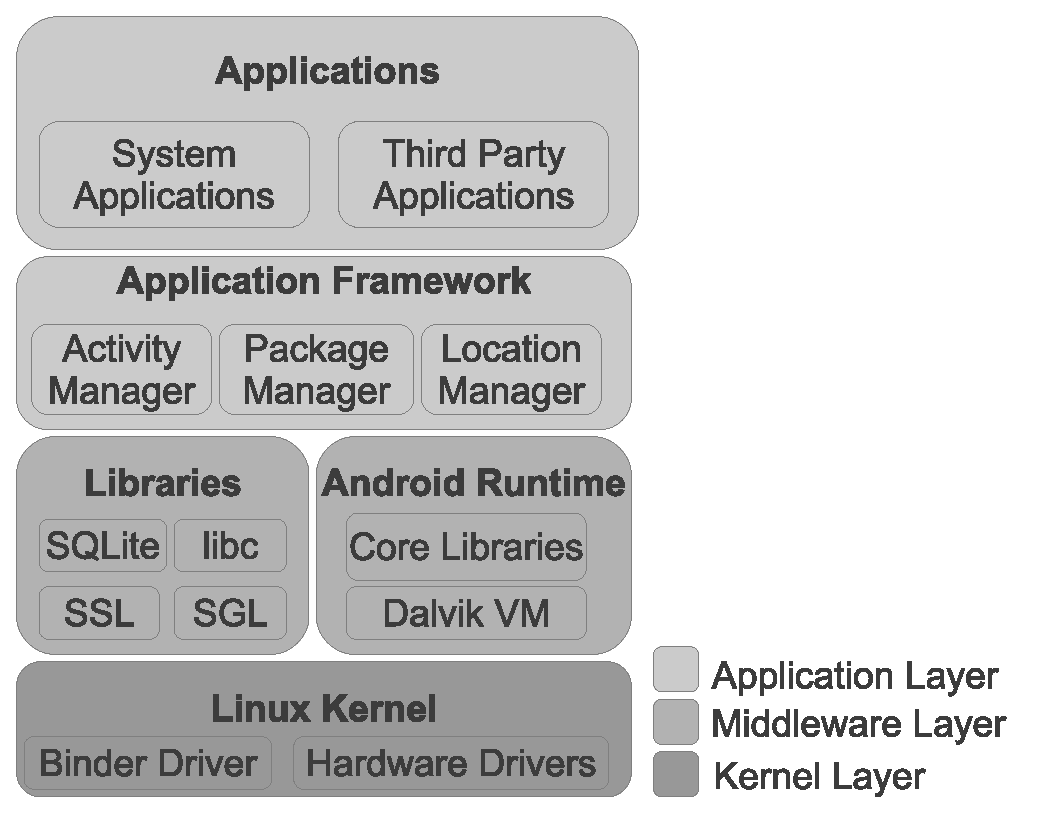
\psfig{file=android_arch.eps,width=2.0in}
\caption{Android Software Stack}
\label{fig:android}
\end{figure}

%The Linux-based kernel is located at the lowest layer of the 
%Android software stack. 
The kernel is responsible for providing 
the core functionality of Android, such as process management, 
networking, memory management, and device drivers to allow for 
the software to communicate with the hardware resources. 
Furthermore, the Linux kernel provides Android with the security 
functionality needed to enforce process isolation, hardware 
access privileges, and file access privileges through utilizing 
user identifiers (UIDs), group identifiers (GIDs) and file 
system access permissions.  
%Applications that are installed
%typically have a unique UID, however, Android also allows
%applications that are signed with the same signature to share
%a UID to allow two different applications to access each others
%resources (e.g., files).  However, since applications typically
%run in an isolated process under a unique UID, Android includes
%a mechanism in the Linux kernel (Binder) that allows
%inter-process communication.

%The middleware layer is located above the kernel layer of the 
%Android software stack, which 

The middleware consists of the native libraries 
and the runtime environment. The native libraries provide the 
system with machine independent functionality, such as the \textit{libc} 
library, a SSL implementation, and an SQLite implementation. 
The runtime environment consists of the core libraries and the 
Dalvik virtual machine. The core libraries provide the system 
with an implementation of the Java API, the Android libraries, 
and the Dalvik Virtual Machine's libraries. The Dalvik Virtual 
Machine is a process-level virtual machine that is responsible 
for executing Android applications that were compiled into 
Android's custom bytecode (DEX). 
%The middleware layer also 
%provides the system with a reference monitor that enforces 
%mandatory access control (MAC) for inter-component 
%communications.

%The application layer is located at the top of the Android 
%software stack and 
The application layer contains the application framework and 
applications. The application framework provides Android 
application developers with basic blocks with which 
applications directly interact.
%, such as the activity manager,
%package manager, location manager, and content providers.
%Applications are at the very top of the Android software stack
%and provides the user with software to perform specific tasks,
%such as a contact manager, a web browser, or a text messaging
%interface.  
Android applications are distributed as an application
package file (APK), which contains a manifest file that declares
the application's requested permissions and components, the DEX
bytecode of the application, resources, and application
certificates.  Applications may also define their own custom
permissions in the manifest file to enforce access control
policies on the components or data that they expose to other
applications.  Furthermore, applications may either be
\textit{system applications} (signed with the same signature
as the system image) or \textit{third-party applications}.

The access control policies of applications in the Android
system are achieved through the static installation-time
permission model, which are declared in the application's
manifest file and enforced by the reference monitor in the
middleware layer or by the Linux kernel.  
%An application's
%request to access sensitive data (e.g., a user's contacts)
%or hardware resources (e.g., the microphone, camera, etc.)
%must be granted by the user at the time of the application's
%installation.  Once the requested permissions are approved
%and the application is installed, the application will always
%be granted these permissions.

\subsection{Limitations of the Android Security Model}

While Android's permission-based security model suffices for
most applications, these static access controls can not address
the security requirements of applications targeted towards
the healthcare industry.

First, Android's current permission model does not support the
dynamic restriction of an application's privileges.  Since PHI
is not limited to medical records and images (e.g., MRI images),
but rather includes conversations between a doctor and a patient
during an appointment, malicious applications may exploit the
environment in which the mobile device is located to gather PHI
instead of attempting to steal data stored on the device.  For
example, a doctor may download a third-party voice memo recorder
to record reminders of non-sensitive information.  However, the
application may be malicious and launch a background service to
secretly record conversations that include details of PHI and
transmit the recorded audio to an external server.  Therefore,
a mechanism to dynamically restrict an application's privileges
is necessary to prevent the exposure of PHI by malicious
applications.

Second, Android's current framework also lacks the
system-level mechanism that is required to enforce security
policies on PHI data flows and revoke access to PHI.  Due to
the sensitivity of PHI, the system is required be able to
identify and revoke access to the PHI and enforce security policies
on the data (e.g., whether the PHI can be saved or forwarded).
On Android's current framework the organization loses
control the PHI once it is sent to the device, which is
unacceptable when dealing sensitive data.

\subsection{Addressing the Limitations of the Android Security Model}

%To address the limitations of Android's existing security model and
%the previously discussed security challenges for deploying mobile
%devices in the healthcare industry, 
DASF consists of three new
modifications to the Android platform. 

First, DASF provides a system-level mechanism for dynamically
enforcing system-wide privilege restrictions on applications.
Applications can programmatically impose dynamic system-wide privilege
restrictions on other applications if they request permission to
restrict a privilege.

Second, DASF utilizes dynamic taint tracking to identify sensitive
data and track the propagation of the sensitive data throughout
the system. To ease our implementation, this study utilizes
TaintDroid~\cite{taintdroid} to provide
the mechanism for tagging data and propagating the data's tag
throughout the system.  
%Further, we also leverage CleanOS'~\cite{Tang_osdi12} 
%extension of TaintDroid to provide the mechanism
%for revoking sensitive data.  
DASF uses the data's privacy
tags to enforce system-level security policies on the sensitive
data.  DASF augments these models by allowing
system-level security policies to be imposed on the data
(e.g., preventing the data from being saved or forwarded).

Third, we designed a application-layer message protocol at the
system-level that operates over an SSL connection to tag sensitive
data that is received from the server to allow the server to
impose system-level security policies on the data that it sends
to the device.  Further, our message protocol also allows the
server to dynamically impose system-wide privilege restrictions
on applications running on the device.

%Therefore, our contributions are providing system-level support for
%classifying sensitive data and enforcing security policies on that
%sensitive data, and allowing a server, or an application, to dynamically
%enforce system-wide privilege restrictions on the device.

